\documentclass[10pt]{article}
\usepackage{icmlko}

\icmlmeta{IP 파운데이션 월드모델}{349}{달력을 아홉 군데서 뗐다}{노트 341이 빼기는 안 된다고 했는데 아홉 배 크게 빼니 됐다 --- 뺀 데가 더 오른다}

\begin{document}

\twocolumn[
\icmlheader

\begin{abstract}
노트 348이 ``묶음으로 재고 묶음으로 버리지 마라''를 세우고 ``묶음을 다
풀어 보라''를 남겼다. 계열 넷 중 풀 수 있는 것은 \textbf{달력} 하나다 ---
태그는 이미 도메인 전용이고 검색은 아홉 도메인에서 이긴다.

노트 342의 지도가 달력을 이렇게 적었다.

\begin{center}\footnotesize
\begin{tabular}{lrl}
\hline
도메인 & 검사 ⑤ & \\
\hline
\textbf{펀딩} & $+$0.0939 & 8/8 \\
\textbf{웹툰} & $+$0.0474 & 8/8 \\
\hline
팝업 & $-$0.0337 & 1/8 \\
도서 & $-$0.0235 & 2/8 \\
아이돌 & $-$0.0212 & 4/8 \\
모바일 & $-$0.0065 & 1/8 \\
\hline
\end{tabular}
\end{center}

\textbf{이기는 둘만 남기고 아홉에서 뺐다} --- 축 여섯 $\times$ 도메인 아홉
$=$ \textbf{쉰네 칸}.

\begin{center}\small
\begin{tabular}{lrr}
\hline
 & 판 & 양수 \\
\hline
\textbf{달력을 둘만} & \textbf{$+$0.0044} & \textbf{11/12} \\
\hline
\end{tabular}
\end{center}

\textbf{올랐다} --- 그리고 \textbf{뺀 데가 더 오른다}: 도서
$+$0.0398(11/12) · 아이돌 $+$0.0360(10/12) · 팝업 $+$0.0269(11/12) ·
모바일 $+$0.0097(11/12). 달력을 \emph{남긴} 펀딩 $+$0.0071 · 웹툰
$+$0.0030 보다 크다.

\textbf{미리 적은 것이 틀렸다.} 노트 341이 위키를 진 두 도메인에서 빼고
판 $+$0.0009(7/12)를 얻어 ``빼기는 붙이기의 역이 아니다''로 끝냈고, 나는
그걸 근거로 ``이번에도 안 오를 것''이라 적었다. \textbf{그때는 도메인 둘
$\times$ 축 셋 $=$ 여섯 칸이었고 이번은 쉰네 칸이다} --- \textbf{빼기도
값이 있는데 충분히 커야 보인다.}

배포 규칙 ①②를 통과한다(제일 나쁜 애니 $-$0.0075 · 짝SE 0.006 ·
$t{\approx}1.25$). \textbf{판 0.4815 $\to$ 0.4859.}
\end{abstract}
]

\section{풀 수 있는 것은 달력뿐}

\begin{center}\footnotesize
\begin{tabular}{ll}
\hline
계열 & 왜 못 푸나 \\
\hline
태그 & 이미 도메인 전용 --- 자를 것이 없다 \\
검색 & 아홉에서 이기고 팝업만 $-$0.0007(4/8) \\
위키 & 노트 341이 이미 해 봤다(둘 $\times$ 셋) \\
\textbf{달력} & \textbf{전 도메인 100\% 인데 둘만 이긴다} \\
\hline
\end{tabular}
\end{center}

\begin{figure*}[t]
\centering
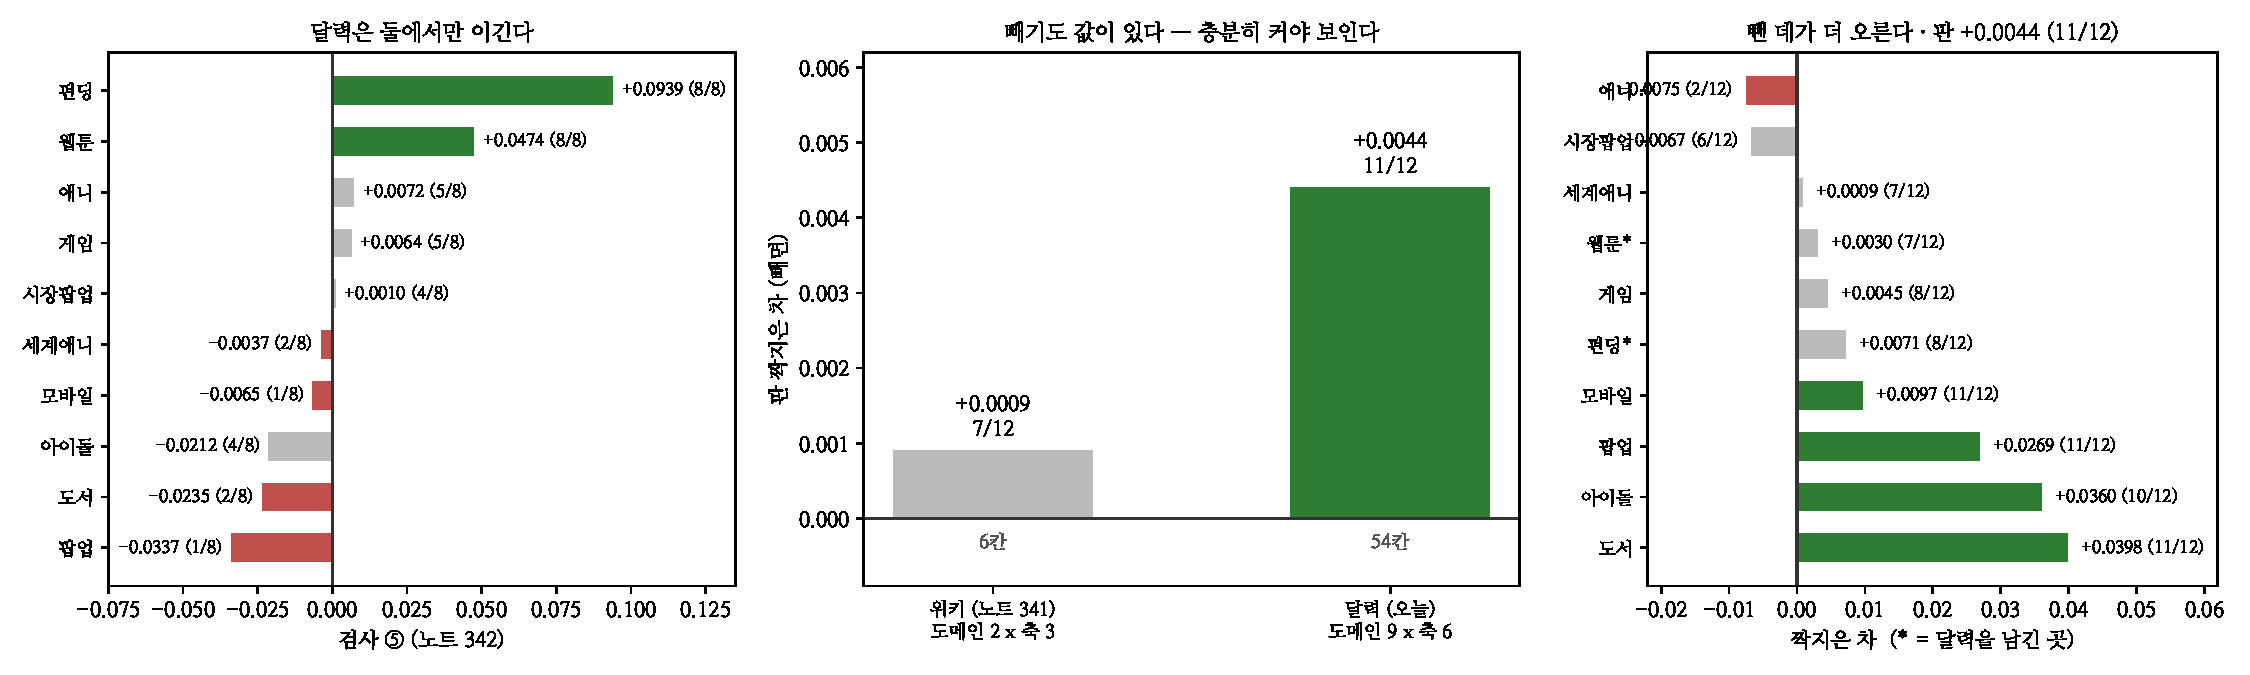
\includegraphics[width=\textwidth]{figs/calcut.pdf}
\caption{왼쪽 --- 달력의 검사 ⑤ 지도. 가운데 --- 빼기의 규모.
오른쪽 --- 붙인 결과.}
\end{figure*}

\section{뺀 데가 더 오른다}

\begin{center}\footnotesize
\begin{tabular}{lrrl}
\hline
도메인 & 평균 & 양수 & \\
\hline
도서 & $+$0.0398 & 11/12 & 뺌 \\
아이돌 & $+$0.0360 & 10/12 & 뺌 \\
팝업 & $+$0.0269 & 11/12 & 뺌 \\
모바일 & $+$0.0097 & 11/12 & 뺌 \\
펀딩 & $+$0.0071 & 8/12 & \textbf{남김} \\
웹툰 & $+$0.0030 & 7/12 & \textbf{남김} \\
시장팝업 & $-$0.0067 & 6/12 & 뺌 \\
애니 & $-$0.0075 & 2/12 & 뺌 \\
\hline
\textbf{판} & \textbf{$+$0.0044} & \textbf{11/12} & \\
\hline
\end{tabular}
\end{center}

\textbf{남긴 둘은 거의 안 움직이고 뺀 넷이 크게 오른다.} 남긴 곳은 원래
쓰던 것을 그대로 쓰니 당연하고, \textbf{뺀 곳은 안 쓰던 열이 사라지면서
나무가 다른 데를 본다.} 노트 339가 ``무작위 축 하나가 판을 0.126
내린다''고 잰 그 값이 여기서 도메인마다 회수된다.

\paragraph{애니만 내려간다} $-$0.0075(2/12). 노트 342에서 애니는 달력이
$+$0.0072(5/8)로 못 가르는 자리였다 --- \textbf{지도가 ``못 가른다''로
적은 곳을 뺐더니 손해가 났다.} 지도의 0 은 0 이 아니었다.

\section{빼기의 규모}

\begin{center}\small
\begin{tabular}{lrrr}
\hline
 & 칸 & 판 & 양수 \\
\hline
위키(노트 341) & 6 & $+$0.0009 & 7/12 \\
\textbf{달력}(오늘) & \textbf{54} & \textbf{$+$0.0044} & \textbf{11/12} \\
\hline
\end{tabular}
\end{center}

\textbf{아홉 배 크게 빼니 다섯 배 올랐다.} 노트 341의 결론(``검사 ⑤ 는
붙일까에 답하지 뺄까에는 답하지 않는다'')을 고친다 --- \textbf{답하는데
한 번에 조금 빼면 안 보인다.} 노트 338이 ``차이도 한 번 재면 안 된다''를
세웠는데, 여기서는 \textbf{차이가 너무 작아서 안 보였다.}

\section{남은 것}
\begin{center}\footnotesize
\begin{tabular}{ll}
\hline
갈래 & 왜 \\
\hline
\textbf{애니에 달력을 되돌릴까} & 지도의 0 이 0 이 아니었다 \\
검색도 팝업에서 뺄까 & 하나뿐이라 작다 \\
위키를 다시 크게 & 진 자리가 지금은 다를 수 있다 \\
남은 축을 한 번에 훑어 & 지도를 다시 그려라 \\
\hline
\end{tabular}
\end{center}

\paragraph{규약} \textbf{처치가 안 보이면 처치를 키워 보라.} 노트 341이
위키를 두 도메인에서 빼고 $+$0.0009 를 얻어 ``빼기는 값이 없다''로 읽었다.
같은 일을 아홉 배로 하니 $+$0.0044(11/12)다. \textbf{``효과가 없다''와
``효과가 잰 것보다 작다''는 다른데, 한 번의 작은 처치로는 그 둘을 못
가른다.} 그리고 이 판에서 처치를 키우는 것은 대개 공짜다 --- 같은 코드에
도메인을 더 넣으면 된다.

\end{document}
